% !TeX spellcheck = en_US

\chapter{Practical Results}\label{chp:practical_results}

\section{QGIS Plugin}
A QGIS plugin has been created, which allows to process the currently displayed imagery in a corresponding backend server. \autoref{fig:plugin:changes} shows an image of the imagery layer overlayed with the changes generated by the backend. The red dots on the upper left indicate deleted objects, or in other words, buildings that were not predicted in the image but were existent at the same location in the cadastral survey data. However, it is obvious, that in this case the neural network is wrong, as the actual buildings can be seen clearly. Additionally, in the lower middle the blue area can be seen, which indicates a change in the survey data.

A prediction is classified as change, as soon as it fully covers at least one existing object in the survey data. \autoref{fig:plugin:changes_cadastral_layer} shows the same changes on the cadastral data layer and \autoref{fig:plugin:predictions} shows the predictions as returned by the neural network.

\begin{figure}[H]
    \centering
	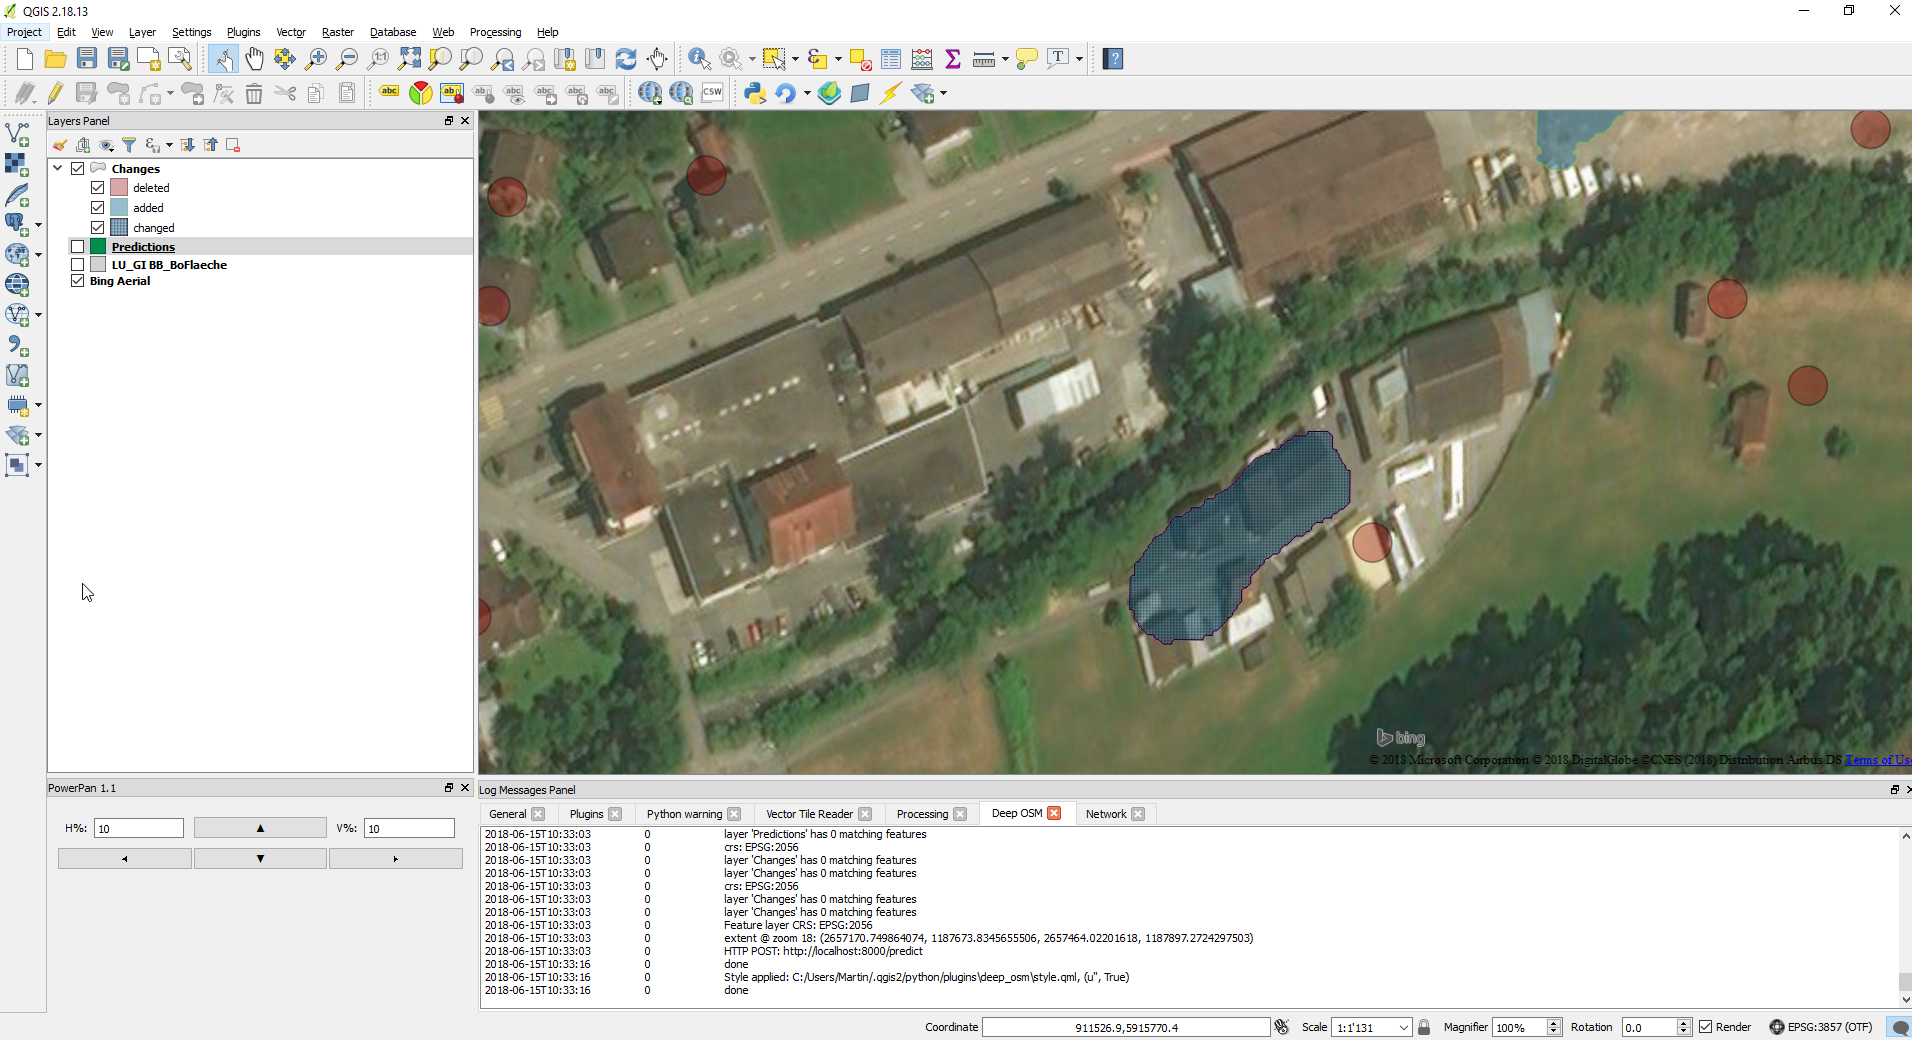
\includegraphics[width=1\linewidth]{chapters/practical_results/images/qgis_changes_aerial.png}
	\caption{Changes in QGIS}
	\label{fig:plugin:changes}
\end{figure}

\begin{figure}[H]
    \centering
	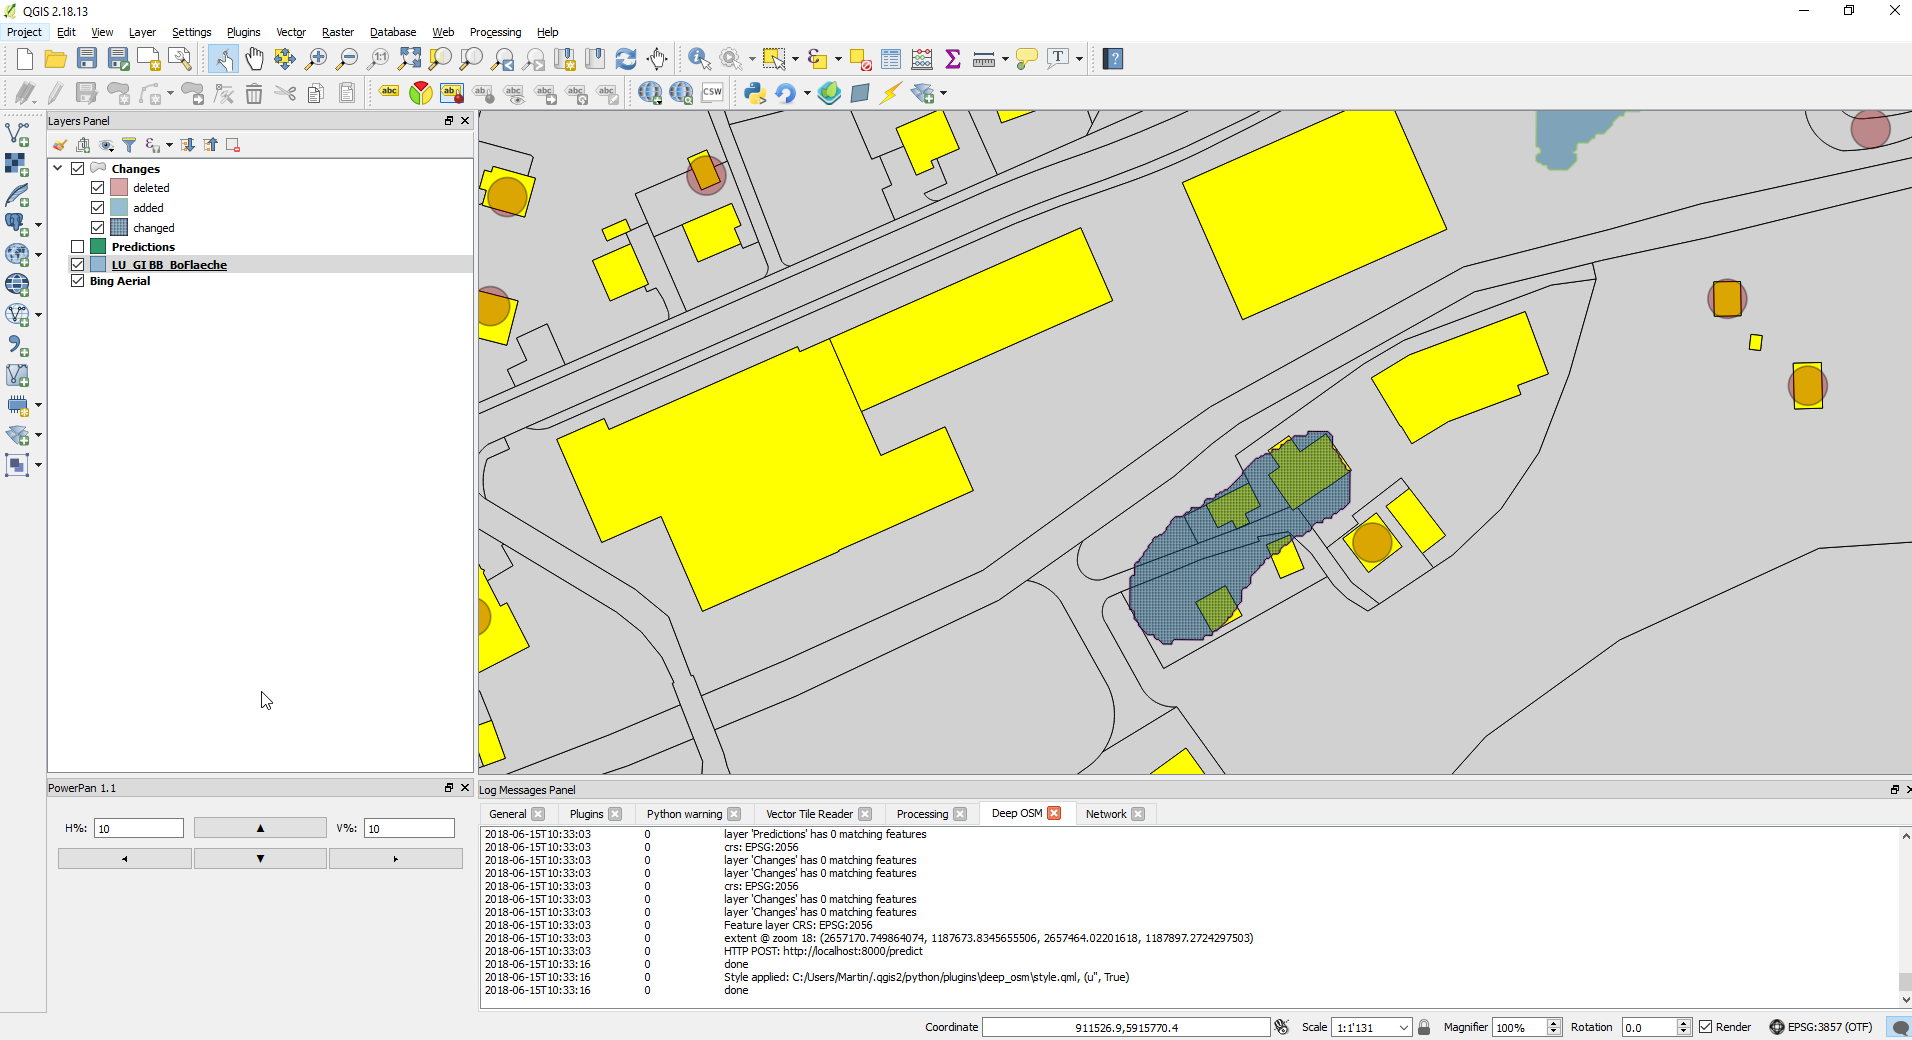
\includegraphics[width=1\linewidth]{chapters/practical_results/images/qgis_changes.png}
	\caption{Changes on cadastral survey data layer}
	\label{fig:plugin:changes_cadastral_layer}
\end{figure}

\begin{figure}[H]
    \centering
	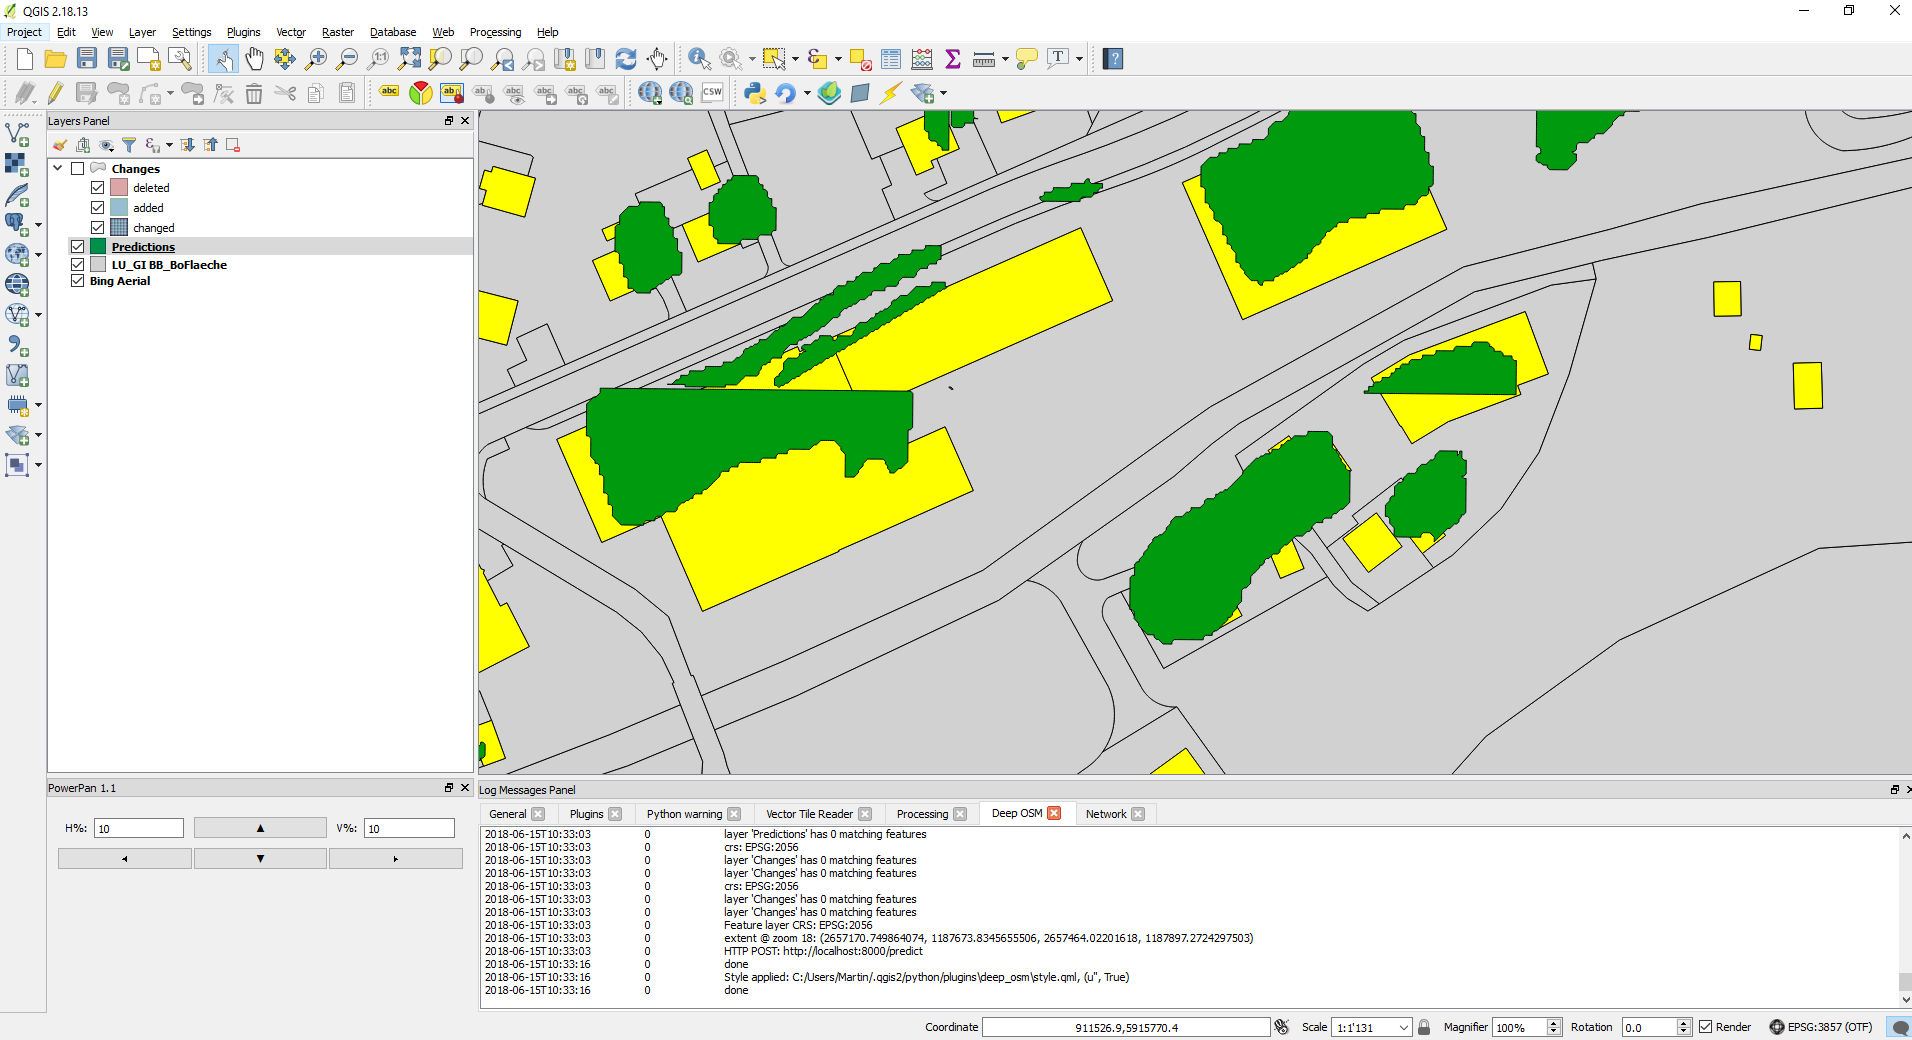
\includegraphics[width=1\linewidth]{chapters/practical_results/images/qgis_predictions.png}
	\caption{Predictions (green) as generated by the neural network}
	\label{fig:plugin:predictions}
\end{figure}

\begin{figure}[H]
    \centering
	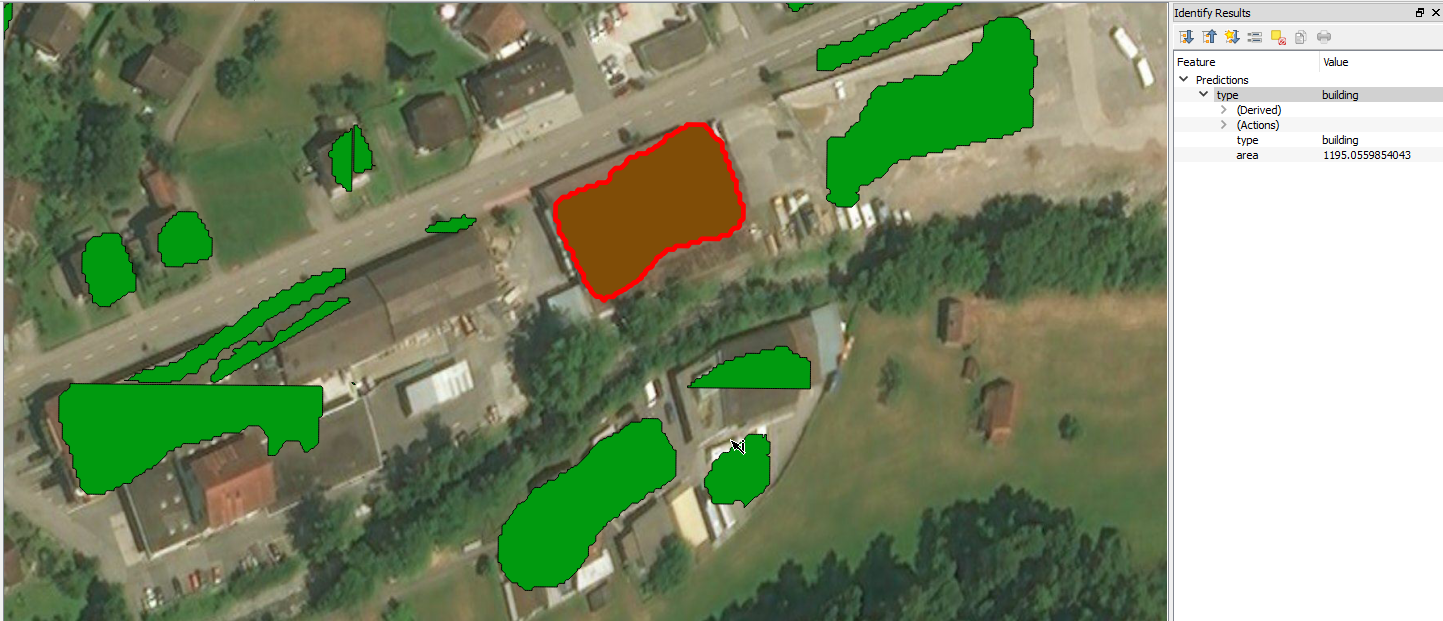
\includegraphics[width=1\linewidth]{chapters/practical_results/images/qgis_prediction_attributes.png}
	\caption{Predictions have attributes showing the predicted class (building in this case)}
	\label{fig:plugin:prediction_attributes}
\end{figure}

\begin{figure}[H]
    \centering
	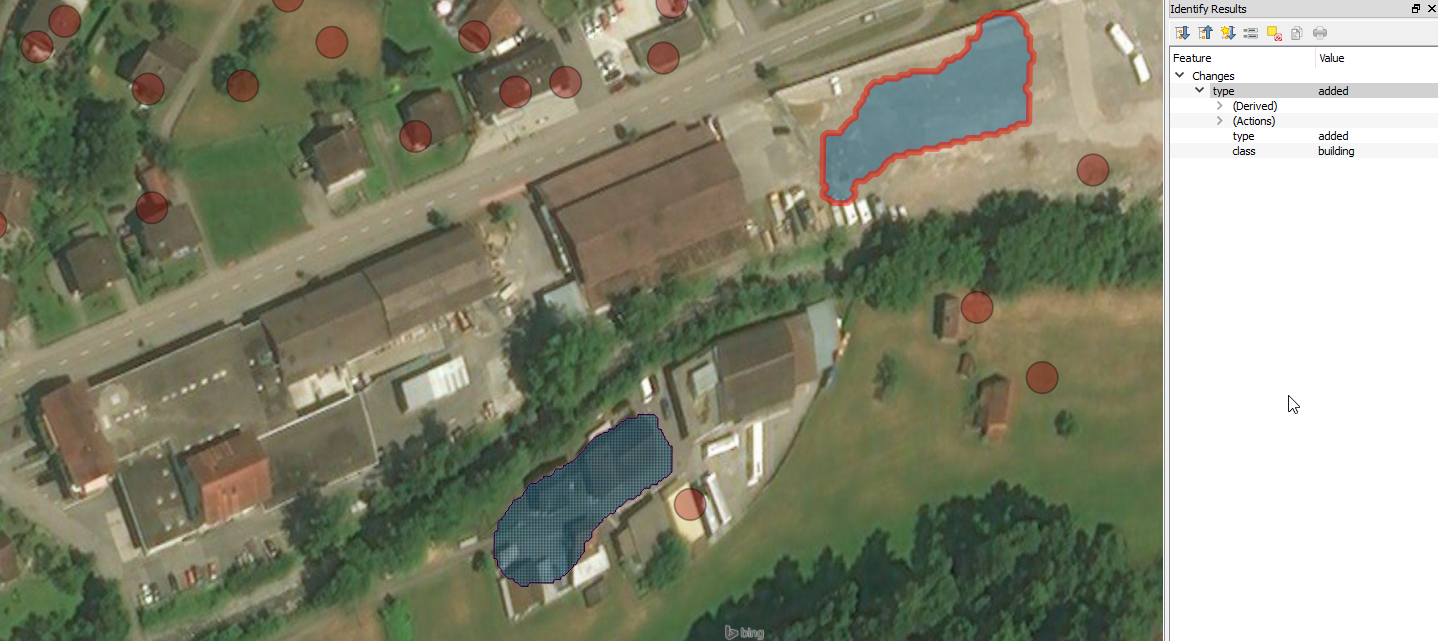
\includegraphics[width=1\linewidth]{chapters/practical_results/images/qgis_changes_attributes.png}
	\caption{Changes have attributes showing the predicted class and the type of change (added, deleted, changed)}
	\label{fig:plugin:change_attributes}
\end{figure}
